\documentclass[USenglish,oneside,twocolumn]{article}

\usepackage[utf8]{inputenc}%(only for the pdftex engine)
%\RequirePackage[no-math]{fontspec}%(only for the luatex or the xetex engine)
\usepackage[big]{dgruyter_NEW}
% allow URL breaks on dashes
\def\UrlBreaks{\do\/\do-}

% math environment
\usepackage{mathtools}
\usepackage{amsmath}
\usepackage{amssymb}
\usepackage[%
    lambda, advantage, operators, sets, adversary, landau, probability, notions,
    logic, ff, mm, primitives, events, complexity, asymptotics, keys,
]{cryptocode}

% prettier line breaks
\usepackage{microtype}

% figures
\usepackage{graphicx}
\usepackage[position=bottom]{subfig}
\usepackage{tikz}
\usepackage{tikz-qtree}
\usetikzlibrary{shapes.misc,positioning,arrows,snakes,calc}

% colors
\usepackage{color}
\usepackage{colortbl}
\definecolor{rgddTeal}{HTML}{009999}
\definecolor{rgddLime}{HTML}{809933}
\definecolor{rgddPurple}{HTML}{993380}
\definecolor{rgddDred}{HTML}{E04644}
\definecolor{rgddDgreen}{HTML}{008000}
\definecolor{rgddDblue}{HTML}{2809B2}

% custom commands
\newcommand{\TODO}[1]{\textcolor{red}{TODO:} \emph{#1}}

 
\DOI{foobar}

\cclogo{
\includegraphics{by-nc-nd.pdf}}
  
\begin{document}
  %\author*[1]{Corresponding Author}
  %\author[2]{Second Author}
  %\author[3]{Third Author}
  %\author[4]{Fourth Author}
  %\author[5]{Fifth Author}
  %\affil[1]{Affil, E-mail: email@email.edu}
  %\affil[2]{Affil, E-mail: email@email.edu}
  %\affil[3]{Affil, E-mail: email@email.edu}
  %\affil[4]{Affil, E-mail: email@email.edu}
  %\affil[5]{Affil, E-mail: email@email.edu}

  \title{\huge CTor: Certificate Transparency in Tor}
  \runningtitle{CTor: Certificate Transparency in Tor}
  %\subtitle{...}

  \begin{abstract}
      {The security of the web has greatly improved in the last couple of years. HTTPS
is now the default, with browsers moving towards warning when unencrypted
connections are made. The Certificate Authority (CA) system has also improved.
The advent of mandatory Certificate Transparency (CT) logging of all
certificates issued by CAs---enforced by web browsers---has made the
weakest-link setting of the CA system more sustainable. However, Tor and its Tor
Browser, based on Firefox, is missing support for CT.

In this paper, we present designs for privacy preserving and
incrementally-deployable support for CT in Tor. Our designs go beyond
the support for CT found in browsers like Google Chrome or Apple's
Safari: we aim to do more than detect CA misbehavior supporting
man-in-the-middle or impersonated HTTPS connections from Tor Browser.
We also create independent public evidence of CT log misbehavior in
support of this. Our base design shares observed certificates in Tor
Browser with other CT logs. Associated privacy leaks of browsing
behavior of Tor users are minimized through the use of indirect
routing and randomized delay of certificate reporting through relays
in the Tor network.

We also present two possible extensions to our base design that can also detect
CT log misbehavior. One extension makes a slight change to the API and operation
of CT logs, the other adds more complexity to Tor but in turn completely removes
all trust placed in CT log operators. Detecting CT log misbehavior is
particularly important for the wider web, since CT as currently deployed lacks
strong mechanisms necessary for reducing trust in CT log operators.
We turn Tor into a system for maintaining a probabilistically-verified view of
the CT log ecosystem as available from Tor’s consensus.
}
  \end{abstract}

  \keywords{Certificate Transparency, Tor}
  %\classification[PACS]{}
  %\communicated{...}
  %\dedication{...}

  \journalname{Proceedings on Privacy Enhancing Technologies}
  \DOI{Editor to enter DOI}
  \startpage{1}
  \received{..}
  \revised{..}
  \accepted{..}

  \journalyear{..}
  \journalvolume{..}
  \journalissue{..}
 
  \maketitle
  \section{Introduction} \label{sec:introduction}
Metrics reported by Google and Mozilla reveal that encryption on the web
skyrocketed the past couple of years: at least 85\% of all web pages load using
Transport Layer Security (TLS) as part of
HTTPS~\cite{google-metrics,mozilla-metrics}. An HTTPS connection is initiated by
a TLS handshake where the client web browser requires that the web server
presents a valid certificate to authenticate the identity of the server (e.g.,
to make sure that the client who wants to visit \url{mozilla.org} really is
connecting to Mozilla, and not, say, Google). A certificate is considered valid
if it is digitally signed by a Certificate Authority (CA) that the browser
trusts. Each CA is trusted to certify (sign) that specific cryptographic
key-material as part of a certificate belongs to a particular domain name.

The CA trust model suffers from \emph{weakest-link} security: web browsers trust
hundreds of CAs, and it is enough to compromise a single CA to get a certificate
mis-issued in the name of a target domain~\cite{ca-ecosystem,https-sok}.
Motivated by this issue manifested by prominent CA compromises---such as the
issuance of a fraudulent certificate for \url{google.com} by DigiNotar in
2011\footnote{\url{https://web.archive.org/web/20200521135444/https://arstechnica.com/information-technology/2011/08/earlier-this-year-an-iranian/}}---several
major browser vendors have mandated that certificates issued by CAs must be
included into trusted Certificate Transparency (CT) logs for browsers to trust
them~\cite{ct/a,ct,ct/bis}. The idea behind CT is that, by making all issued
certificates transparent, mis-issued certificates can be detected \emph{after}
issuance and appropriate actions taken to keep the wider web safe (e.g.,
revocation of certificates, suspected compromises investigated, or trust in
misbehaving CAs removed from browsers). Browsers that wish to benefit from CT
augment the validation done by the browser during the TLS handshake to also
require cryptographic proof from the server that the presented certificate has
been included into CT logs trusted by the browser. Notable browsers with
mandatory CT support by default are Google Chrome and Apple's Safari
\cite{chrome-policy,safari-policy}. Unfortunately, Mozilla's Firefox lacks
support but has a partial implementation.

Beyond security on the web, anonymous access to the web has also matured. In
particular, Tor with its Tor Browser (TB) today have millions of daily users
\cite{tor,mani}, and effort is ongoing into maturing the technology for wider
use\footnote{\url{https://web.archive.org/web/20200528174708/https://mozilla-research.forms.fm/mozilla-research-grants-2019h1/forms/6510}}.
The basis of TB is Firefox, where TB then enables anyone to browse the web
anonymously by relaying traffic between browser and web server through the Tor
network, consisting of thousands of voluntary-run relays across the globe. 

Just like attackers may be interested in breaking HTTPS, attackers are
interested in breaking the anonymity provided by Tor with the goal of
deanonymizing users. One common deanonymization technique, known to be used in
practice by, e.g., law enforcement, is to compromise TB instead of directly
circumventing the anonymity provided by the Tor
network\footnote{\url{https://web.archive.org/web/20200528175225/https://zerodium.com/tor.html}}.
Modern web browsers like TB (Firefox) are one of the most complex types of
software in wide use today. This complexity and wide use leads to security
vulnerabilities and incentives for exploitation. For example, the exploit
acquisition platform Zerodium offers up to \$100,000 for a zero-day exploit
against Firefox that leads to remote code execution and local privilege
escalation\footnote{\url{https://web.archive.org/web/20200521151311/https://zerodium.com/program.html}}
(i.e., full control of the browser for the attacker).

An attacker that wishes to use such an exploit to compromise and then ultimately
deanonymize a TB user has to deliver the exploit to TB\@. Since the web is
mostly encrypted today, this primarily has to happen over an HTTPS connection,
where the attacker controls the content returned by the web server. While there
are a number of possible ways for an attacker to accomplish this (e.g., by
compromising a web server that the target TB user connects to), one option is to
\emph{impersonate} a web server by acquiring a fraudulent certificate. Due to
the Tor network being run by volunteers, getting into a position for performing
such an attack is relatively straightforward (the attacker can volunteer to run
malicious relays~\cite{spoiled-onions}). The same is true for an attacker that
wishes to \emph{man-in-the-middle} connections made by TB users. In such a case,
a TB exploit may not even be needed to deanonymize the user; e.g., if the user
logs into an account at the service associated with its identity and that the
attacker can now observe.

\subsection{Introducing CTor}
In this paper, we propose an incremental design which we refer to as CTor. CTor
brings CT to Tor by modifying both how TB and relays in the Tor network work.
The goal is to make impersonation and man-in-the-middle attacks on HTTPS
connections \emph{detectable after the fact} when they are carried out by a
powerful attacker that:
\begin{itemize}
	\item can acquire a forged certificate from a trusted CA,
	\item with the necessary forged cryptographic proofs from CT logs so that TB
	accepts the certificate as valid (with no intent of making the forged
	certificate publicly available in a CT log), and
	\item has the capability to fully gain control of TB shortly after the
	establishment of the HTTPS connection.
\end{itemize}

Our base CTor design uses the CT log ecosystem against the attacker to ensure a
non-zero (tweakable) probability of detection of the forged certificate. This is
done by probabilistically adding the certificate to \emph{other CT logs} than
those directly inferable as under attacker control (due to the accompanying
proofs). TB uses modified relays to cache and interact with CT logs for the sake
of privacy, ensuring that CT log operators (such as Google and Cloudflare) do
not get a real-time feed of all browsing activities from TB (beyond what their
privileged position on the Internet already provides them~\cite{TorDNS}). 
% FIXME: some other source would be good above, have to mention DNS to make
% current one make sense

Beyond the base CTor design we present two extensions. Both extensions have in
common that their goal is to make transparent the forged cryptographic proofs
from attacker-controlled CT logs used to get TB to accept malicious HTTPS
connections. Such a proof would likely immediately disqualify each offending CT
log and thus come and great cost to the attacker in terms of lost capability.
Even a small probability of detection may entail unacceptable risk at such a
high cost. Note that we have already observed several instances of CT logs that
misbehaved~\cite{izenpe-disqualified,venafi-disqualified,gdca1-omission}. Most
recently, a compromised CT log signing key was reported for the first
time~\cite{digicert-log-compromised}. 

The key change in the first extension is that relays now challenge CT logs to
cryptographically prove the correctness of their prior proofs presented to TB
instead of simply sharing the certificates (the subject of the proofs) with
other CT logs. In case an offending CT log fails to provide such a proof
in a timely manner,
the querying relay ensures that the proof arrives at a trusted auditor. While
this adds both more complexity and operational challenges to Tor (of both
auditors and storage at relays), it completely removes all trust in the CT
ecosystem. Another benefit is that, as a consequence of CTor's design, Tor would
provide a probabilistically-audited cryptographically-verifiable view of the
entire CT log ecosystem. This significantly addresses one of the main open
issues with the currently deployed CT ecosystem: the lack of a sufficiently
secure gossiping mechanism that makes it possible to place zero-trust in the log
operators.

The second extension involves only a minor tweak to the base CTor design.
Unfortunately, this tweak is primarily not to Tor but to the API of CT logs.
While similar changes have been discussed earlier in the context of gossiping in
CT, it is a significant deployment issue. The small tweak is that CT logs
provide an API for receiving cryptographic proofs made by other CT logs wrt
certificate inclusion. This would then mean that relays would add to
other CT logs proofs observed by TB clients in addition to the certificate.
This would also significantly reduce the trust assumptions the wider web has to
place on CT log operators, from close to full trust as-is today to only trusting
that some operators are honest.

\subsection{Contribution and Structure}
Section~\ref{sec:background} provides necessary background on CT and Tor. Our
threat model is described in detail in Section~\ref{sec:adversary}, taking into
account the threat models of both Tor and CT\@.

Section~\ref{sec:base} presents the base design of CTor that enables TB to
probabilistically provide evidence to CT logs that it has been presented with a
fraudulent certificate. This greatly impacts risk-averse attackers, since part
of its fraudulent behavior has been made transparent through the CT ecosystem:
the issuing CA may get revoked from the trust store of browsers, the domain name
in question (as part of the certificate) is made public, and awareness of the
event may draw unwanted attention. Our security analysis, in
Section~\ref{sec:analysis}, shows that one of the best bets for an attacker may
be to attack the entire Tor network: an act that in itself may draw unwanted
attention.

Two extensions to the base CTor design are presented in
Sections~\ref{sec:auditor} and \ref{sec:log}. Both extensions aim to make
transparent the accompanying fraudulent proofs issued by CT logs to convince TB
to accept a fraudulent certificate. The deployment of either design would
greatly contribute to the open question of how to reduce trust in CT log operators
currently caused by the lack of an appropriate gossiping mechanism~\cite{FIXME}.
In particular, the auditor-based design (Section~\ref{sec:auditor}) would result
in a probabilistically-audited cryptographically-verifiable view of the entire
CT log ecosystem available from Tor's consensus. This view could be used as the
basis for trust by other browsers, greatly improving the security posture of the
entire web.

Section~\ref{sec:performance} estimates performance aspects of our designs,
including estimated circuit overhead and estimated load on the Tor network.
Privacy aspects of our design choices are covered in Section~\ref{sec:privacy},
with a focus on the essential role of the distributed nature of the Tor network
in both preserving privacy of Tor users as well as the overall security of our
proposed designs. In gist, a similar approach would not work without Tor, e.g.,
if integrated into Google Chrome. Finally, Section~\ref{sec:related} covers
related work and Section~\ref{sec:conclusion} concludes this paper.

%%% Local Variables: 
%%% mode: latex 
%%% TeX-master: "../main"
%%% End:          

  \section{Background} \label{sec:background}
The theory and current practise of CT is introduced first, then Tor
and its privacy-preserving Tor Browser.

\subsection{Certificate Transparency} \label{sec:background:ct}
The idea to transparently log TLS certificates emerged at Google in response to
a lack of proposals that could be deployed without drastic ecosystem changes
and/or significant downsides~\cite{ct/a}.  By making the set of issued
certificate chains\footnote{%
	A domain owner's certificate is signed by an intermediate CA, whose
	certificate is in turned signed by a root CA that acts as a trust
	anchor~\cite{ca-ecosystem}.  Such a \emph{certificate chain} is valid if it
	ends in a trusted anchor that is shipped in the user's system software.
} transparent, anyone that inspect the logs can detect certificate
mis-issuance \emph{after the fact}.  It would be somewhat circular to solve
issues in the CA ecosystem by adding trusted CT logs.  Therefore, the
cryptographic foundation of CT is engineered to avoid any such reliance.
Google's \emph{gradual} CT rollout started in 2015, and evolved from merely
downgrading user-interface indicators in Chrome to the current state of hard
failures unless a certificate is accompanied by a signed \emph{promise} that it
will appear in two independent CT logs~\cite{does-ct-break-the-web}.  Unlike
Apple's CT enforcement~\cite{safari-policy}, one of these logs must additionally
be operated by Google~\cite{chrome-policy}.

The lack of mainstream verification, i.e., beyond checking signatures, allows an
attacker to side-step the current CT enforcement with minimal risk of exposure
\emph{if the required logs are controlled by the attacker}.  
CTor integrates into the gradual CT roll-out by starting on the same
premise of pairwise-independently trusted logs, which
avoids the risk of bad user experience~\cite{does-ct-break-the-web}
and significant system complexity.  For example, web pages are unlikely to
break, TLS handshake latency stays about the same, and no robust management of
suspected log misbehavior is needed.  Retaining the latter property as part of
our incremental designs simplifies deployment.

\subsubsection{Cryptographic Foundation}
The operator of a CT log maintains a tamper-evident append-only Merkle
tree~\cite{ct,ct/bis}.  At any time, a Signed Tree Head (STH) can be produced
which fixes the log's structure and content.  Important attributes of an STH
include
	the tree head (a cryptographic hash),
	the tree size (a number of entries), and
	the current time.
Given two tree sizes, a log can produce a \emph{consistency proof} that proves
the newer tree head entails everything that the older tree head does.  As such,
anyone can verify that the log is append-only without downloading all entries
and recomputing the tree head.  Membership of an entry can also be proven
by producing an \emph{inclusion proof} for an STH.  These proof techniques are
formally verified~\cite{secure-logging-and-ct}.

Upon a valid request, a log must add an entry and produce a new STH that covers
it within a time known as the Maximum Merge Delay (MMD), e.g., 24~hours.  This
policy aspect can be verified because in response, a Signed Certificate
Timestamp (SCT) is returned.  An SCT is a signed promise that an entry will
appear in the log within an MMD.  A log that violates its MMD is said to perform
an \emph{omission attack}.  It can be detected by challenging the log to prove
inclusion.  A log that forks, presenting one append-only version
to some entities and another to others, is said to perform a \emph{split-view
attack}.  Split-views can be detected by STH
gossip~\cite{chuat,dahlberg,nordberg,syta}.

\subsubsection{Standardization and Verification}
The standardized CT protocol defines public HTTP(S) endpoints that allow anyone
to check the log's accepted trust anchors and added certificates, as well as
to obtain the most recent STH and to fetch proofs~\cite{ct,ct/bis}.  For
example, the \texttt{add-chain} endpoint returns an SCT if the added certificate
chain ends in a trust anchor returned by the \texttt{get-roots} endpoint.  We
use \texttt{add-chain} in Section~\ref{sec:incremental}, as well as several
other endpoints in Section~\ref{sec:base} to fetch proofs and STHs.  It might be
helpful to know that an inclusion proof is fetched based on two parameters: a
certificte hash and the tree size of an STH.  The former specifies the log entry
of interest, and the latter with regards to which view inclusion should be
proven.  The returned proof is valid if it can be used in combined with the
certificate to reconstruct the STH's tree head.

The CT landscape provides limited value unless it is verified that the logs
play by the rules.  The rules are influenced by the major browser vendors that
define \emph{CT policies}.  For example, how is CT enforced by their user
agents, and what is required to become a recognized CT log in terms of uptime
requirements and accepted trust anchors.  Google Chrome and Apple's Safari
require that a certificate chain must be accompanied by two independent
SCTs~\cite{chrome-policy,safari-policy}, where independence refers to the
associated log operators.  While there are several ways that a log can misbehave
with regards to these policy aspects, the most fundamental forms of cheating are
omission and split-view attacks.  A party that follows-up on inclusion and
consistency proofs is said to \emph{audit} the logs.

Widespread client-side auditing is a premise for CT logs to be untrusted, but
none of the web browsers that enforce CT engage in such activities yet.  For
example, requesting an inclusion proof is privacy-invasive because it leaks
browsing patterns to the logs, and reporting suspected log misbehavior comes
with privacy~\cite{ct-with-privacy} as well as operational challenges.
Found log incidents are mostly reported manually to the CT policy
list~\cite{ct-policy-mailing-list}.  This is in contrast to automated
\emph{CT monitors}, which notify domain owners
of newly issued certificates based on what actually appeared in the public
logs~\cite{lwm,ct-monitors}.

\subsection{Tor} \label{sec:background:tor}

Most of the activity of Tor's millions of daily users starts with Tor Browser
and connects to some ordinary website via a circuit comprised of three
randomly-selected Tor relays. In this way no identifying information from
Internet protocols (such as IP address) are automatically provided to the
destination, and no single entity can observe both the source and destination of
a connection. Tor Browser is also configured and performs some filtering to resist
browser fingerprinting, and first party isolation to resist sharing state or
linking of identifiers across origins. More generally it avoids storing
identifying configuration and behavioral information to disk.

Tor relays in a circuit are selected at random, but not uniformly. A typical
circuit is comprised of a \emph{guard}, a \emph{middle}, and an \emph{exit}. A
guard is selected by a client and used for several months as the entrance to all
Tor circuits. If the guard is not controlled by an adversary, that adversary
will not find itself selected to be on a Tor circuit adjacent to (thus
identifying) the client. And because some relay operators do not wish to act as
the apparent Internet source for connections to arbitrary destinations, relay
operators can configure the ports (if any) on which they will permit connections
besides to other Tor relays. Finally, to facilitate load balancing, relays are
assigned a weight based on their apparent capacity to carry traffic. In keeping
with avoiding storing of linkable state, even circuits that share an origin will
only permit new connections over that circuit for ten minutes. After that, if
all connections are closed, all state associated with the circuit is cleared.
Similarly, at each relay state associated with a given circuit is cleared
shortly after a circuit is closed.

Tor clients use this information when choosing relays with which to build a
circuit. They receive the information via an hourly updated \emph{consensus}.
The consensus assigns weights as well as flags such as \texttt{guard} or
\texttt{exit}. It also assigns auxiliary flags such as
\texttt{stable}, which, e.g.,
is necessary to obtain the \texttt{guard} flag since guards must have good
availability. Self-reported information by relays in their \emph{extra-info
document}, such as statistics on their read and written bytes, are also part of
the consensus and uploaded to \emph{directory authorities}. Directory
authorities determine the consensus by voting on various components making up
the shared view of the state of the Tor network. Making sure that all clients
have a consistent view of the network prevents epistemic attacks wherein clients
can be separated based on the routes that are consistent with their
understanding~\cite{danezis:pets2008}. This is only a very rough sketch of Tor's
design and operation.  More details can be found by following links at Tor's
documentation site~\cite{tor-documentation}.

Tor does not aim to prevent end-to-end correlation attacks. An adversary
controlling the guard and exit, or controlling the destination and observing the
client ISP, etc. is assumed able to confirm who is connected to whom on that
particular circuit. The Tor threat model assumes an adversary able to control
and/or observe a small to moderate fraction of Tor relays measured by both
number of relays and by consensus weight, and it assumes a large
number of Tor clients
able to, for example, flood individual relays to detect traffic signatures of
honest traffic on a given circuit~\cite{long-paths}. Also, the adversary can
knock any small number of relays offline via either attacks from clients or
direct Internet DDoS. 

  \section{Threat Model} \label{sec:adversary}
%
% Attacker capabilities
%
We consider an attacker that controls
	a CA,
	enough CT logs to pass Tor Browser's SCT-centric CT policy, 
	some Tor clients, and
	a moderate fraction of Tor relays.
For example, it is possible to
	issues certificates and SCTs,
	dishonor promises of public logging,
	present split-views at will,
	intercept and delay traffic from controlled exit relays as well as CT logs,
		and
	be partially present in the network.
Note that this includes a weaker attacker that does not \emph{control} CAs and
CT logs, but, who gained access to their signing
keys~\cite{turktrust,gdca1-omission}.
A subset of CTor entities can be subject to DoS, but not everyone at once and
all the time.  In other words, we consider the threat model of Tor and Tor
Browser as a starting point~\cite{tor,tor-browser}.  It assumed that the
attacker knows all Tor relay configurations, e.g., available memory and setup of
torlog.

%
% Attacker goal and mindset
%
Given that we are in the business of enforcing CT, the attacker needs to hide
mis-issued TLS certificates and SCTs from entities that audit the CT landscape.
As described in Section~\ref{sec:background:ct}, this can either be achieved by
omission or slit-view attacks.  Our intended attacker is clearly powerful and may
successfully issue a certificate chain and associated SCTs without detection
some of the time, but, a CA caught in mis-issuance or a CT log that violated an
MMD promise will no longer be regarded as trusted.  Therefore, we assume a
\emph{risk-averse} attacker that above a relatively low probability of detection
would be deterred from engaging in such activities.

%
% - Our goal: detect TB HTTPS MitM
% - Why: it is a reasonable prerequisite to conduct attacks against TB users
%
We want to minimize the existence of successful man-in-the-middle attacks
against Tor Browser where it cannot be established if
and how they were carried out.  The property of \emph{detection} is inherited
from CT's threat model, which aims to remedy certificate mis-issuance
\emph{after the fact}; not prevent it~\cite{ct/a}.  We
focus on HTTPS traffic that Tor Browser generated because Tor is used to browse
the normal (encrypted) web~\cite{mani}.  Note that it is generally
\emph{difficult} to target a specific Tor Browser user due to Tor's anonymity,
circuit isolation, and HTTPS everywhere.  However, targeting some or all 
users that visit a website is an eminent threat:
	simply intercept traffic from an exit relay or
	upstream of the website.
Once network traffic can be intercepted, it is trivial to serve an exploit to a
subset of Tor Browser users and much easier to target an identifiable user.
Such zero-day exploits are considered in our threat model because \emph{user
exploitation} is the primary reason to attack Tor Browser.

%
% Defer introducing threats that follow from design details
%
We identify additional threats that follow from our adversary model and
design throughout the paper.  For example, the attacker may attempt to
\emph{flood} a Tor relay's submission endpoint to the extent that some
submission must be deleted, i.e., by posing as a Tor Browser user.  If enough
submissions are deleted, the attacker builds up confidence that stored evidence
of CA and CT log misbehavior will not be audited in phase~3
(Section~\ref{sec:todo}).

%%% Local Variables: 
%%% mode: latex 
%%% TeX-master: "../main"
%%% End:          

  \section{Design} \label{sec:design}
Figure~\ref{fig:design-ca} provides an overview of our design idea.  The starting
point is that zero or more certificate chains and SCTs are presented
throughout a website visit (step~1).  We refer to these as SCT Feedback Objects
(SFOs)~\cite{nordberg}.  Tor Browser accepts an SFO if it adheres to an
SCT-centric CT policy similar to Chrome and Safari~%
\cite{chrome-policy,safari-policy}, but it may also be submitted to a CTR
in the background using a fresh independent circuit (step~2).  CTR flags are
assigned by Tor's directory authorities, and among other things, they also
determine Tor's view of the CT landscape by publishing STHs and announcing
third-party CT auditors in the Tor consensus.  CTRs store SFOs temporarily
before challenging the logs to prove inclusion with regards to Tor's published
STHs (step~3).  Should a log fail to provide a valid inclusion proof for an SFO
within a timely manner, it is reported to an auditor that investigates the issue
further (step~4).
\begin{figure*}
	\centering
	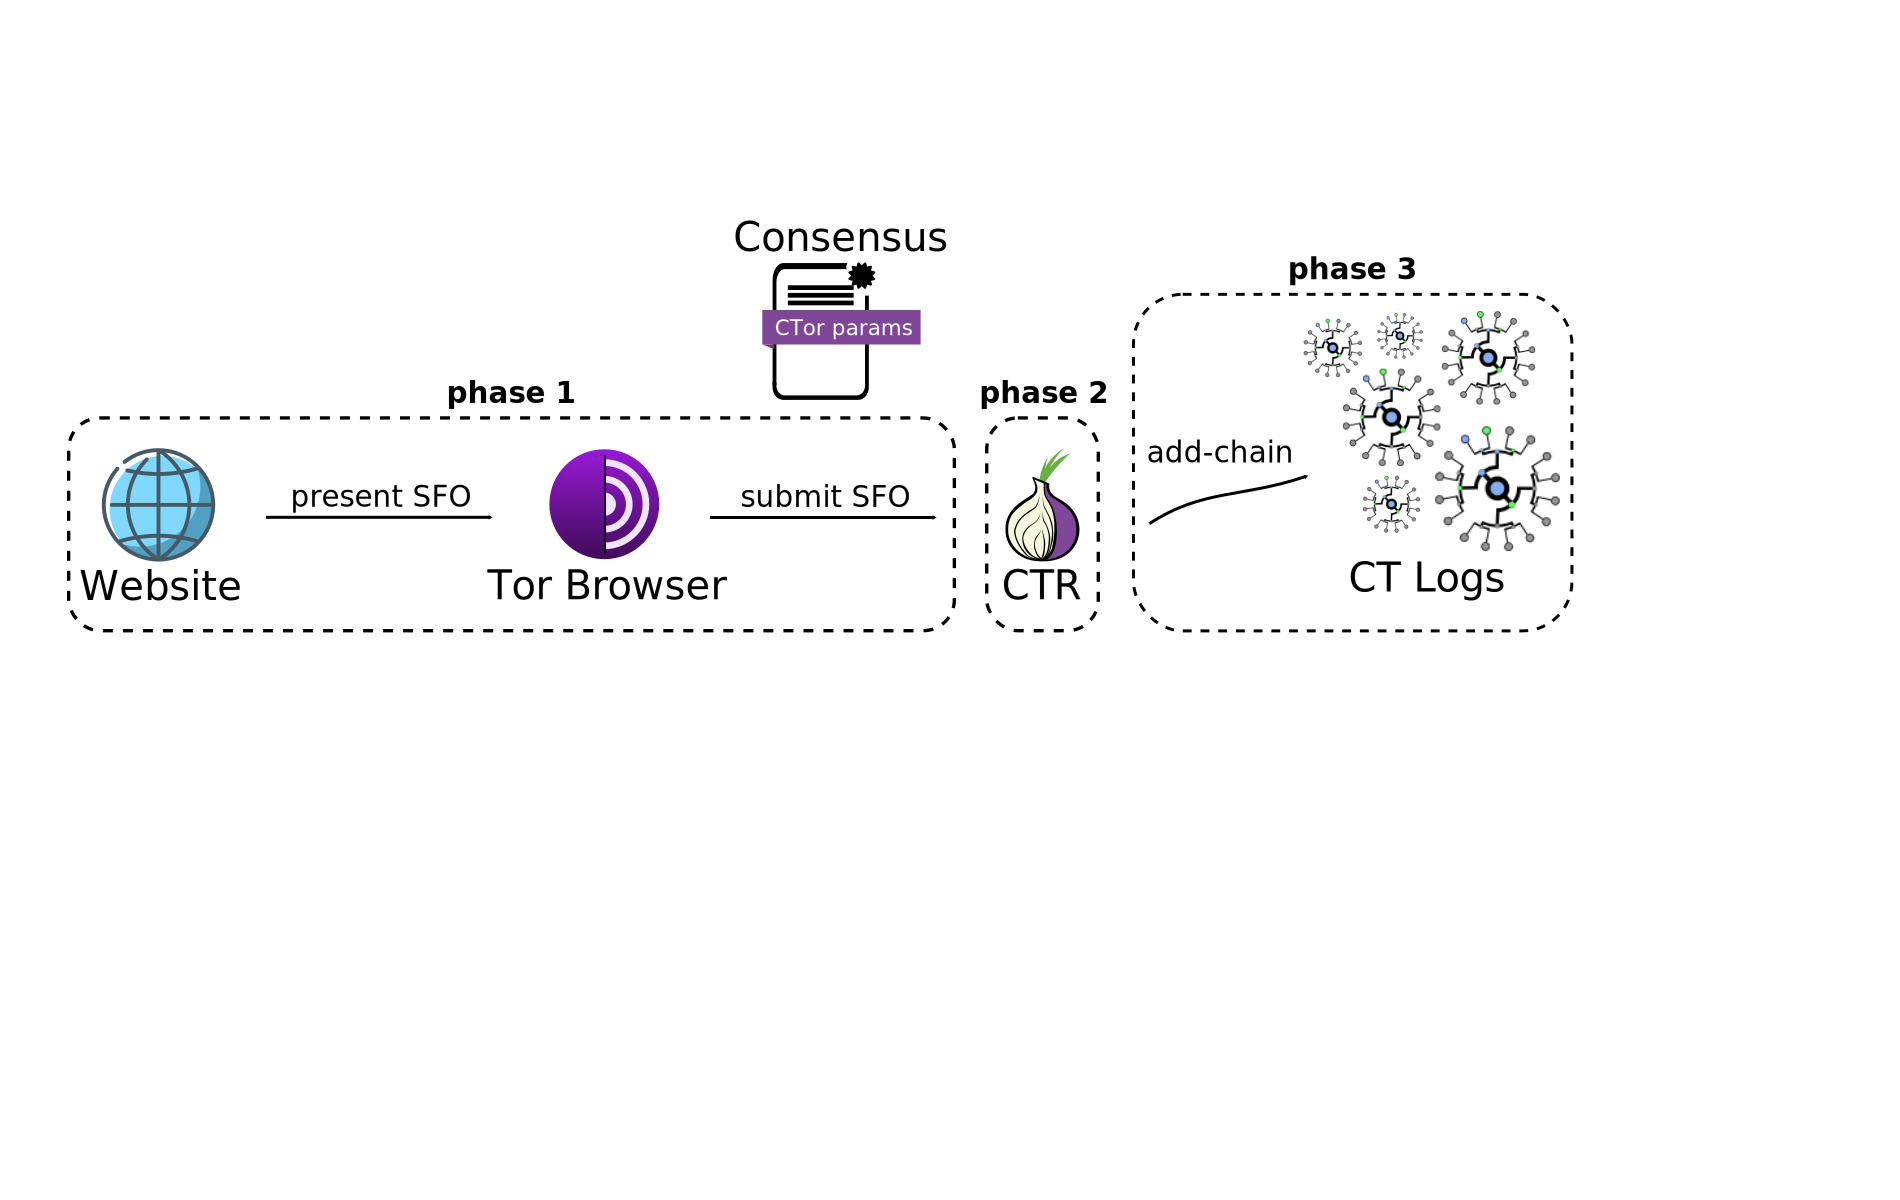
\includegraphics[width=0.85\textwidth]{img/design-ca}
	\caption{An overview of our design: TODO. }
	\label{fig:design-ca}
\end{figure*}

\subsection{Tor Consensus}
Tor's directory authorities produce an hourly consensus document that defines
how the Tor network is composed.  Our proposal extends Tor's consensus document
so that it entails information regarding
	CTRs,
	recognized CT logs,
	announced auditors, and
	security parameters.

\subsubsection{CTR Flag}
The existing \texttt{known-flags} item determines the different flags that a
given consensus document might contain.  For example, documented flags include
\texttt{Authority}, \texttt{Exit}, and \texttt{Running}.  We add another flag
named \texttt{CTR}, which indicates that a relay should support CT-auditing as
described in Section~\ref{sec:design:ctr}.  A relay qualifies as a CTR if it is
flagged as \texttt{stable} and \texttt{middle}.  The \texttt{CTR} flag is
assigned if a majority of directory authorities voted for it.

% - A CTR should be stable both to permit long-lived circuits to the CT logs and
% to increase the likelihood of them staying online.
% - The criteria of being a middle relay, as opposed to an exit relay, follows
% mainly from resource utilization considerations.  It is also about not making
% exit relays "more attractive targets" due to also storing SFOs.

\subsubsection{Recognized CT Log}
The CT landscape is composed of a few dozen logs.  At minimum, the Tor
consensus must recognize those referred by Tor Browser's CT policy.  At some
point during the voting timeline, each directory authority
(i) checks whether there are any CT policy updates, and
(ii) fetches an STH from each log that is recognized.
To agree on a single STH per log, choose the most recent one as determined by
timestamp and resolve ties by appealing to lexicographical order.  A log is
included in the Tor consensus if a majority of directory authorities voted
for it by proposing an instance of \texttt{ct-log-info}:
\begin{description}
	\item[ct-log-info:] Contains a log ID, an MMD and a base URL as found in
		Tor Browser's CT policy, as well as an STH following the log's
		\texttt{get-sth} format~\cite{ct,ct/bis}.
\end{description}

There should be no disagreement regarding a log's basic metadata.  However, if
such an erroneous state occurs, deterministic rules could be used to agree upon
an MMD and a base URL while investigating the issue further.

\subsubsection{Announced Auditor}
Whenever log misbehavior is suspected, the CTR in question reports it to a
CT auditor that investigates the issues further.  Tor's directory authorities
announce CT auditors by proposing a value for the item below, and it is included
in the Tor consensus if a majority of directory authorities voted for it.
\begin{description}
	\item[ct-auditor:] Contains a base URL and a fingerprint that is derived
		from the auditor's public key info.
\end{description}

As built upon in Section~\ref{sec:design:auditor}, the base URL determines the
start of an auditor's submission endpoint.  Moreover, it should be noted that
we pin the auditor's public key because we are dealing with an attacker that
forges TLS certificates.  E.g., a SPKI fingerprint could be used~\cite{hpkp}.

\subsubsection{Security Parameters}
The security of our proposal depends on parameters that Tor's directory
authorities set.  These parameters are first outlined below briefly, then used
throughout the remainder of this section and discussed further later on.
Note that each item occurs exactly once in the Tor consensus:
it is based on the median value of all votes.
\begin{description}
	\item[ct-submit-pr:] A floating-point in $[0,1]$ that determines Tor
		Browser's submission probability, i.e., whether an SFO should be sent to
		a random CTR for further auditing.  E.g., $0$ disables auditing
		while $0.10$ implies every 10$^{\mathsf{th}}$ SFO is audited
		on average.
	\item[ct-submit-timeout:] A natural number that determines how many ms Tor
		Browser waits before concluding that a CTR is unresponsive.  As
		outlined in Section~\ref{sec:design:tb}, a submission timeout results
		in a resubmission to another CTR that is selected at random.
	\item[ct-query-timeout:] A natural number that determines how many ms a CTR
		waits before concluding that a CT log is unresponsive.  As outlined in
		Section~\ref{sec:design:ctr:audit}, a query timeout triggers an
		auditor submission.
	\item[ct-report-timeout:] A natural number that determines how many ms a
		CTR waits before concluding that an announced auditor is unresponsive.
	\item[ct-report-count:] The number of announced auditors that a CTR
		resubmits an SFO to after a report timeout, as well as the number of CT
		logs that the underlying certificate chain is submitted to for public
		logging.  Further details are outlined in
		Section~\ref{sec:design:ctr:audit}.
	\item[ct-backoff:] A natural number that determines how many ms a CTR
		may wait between two auditing instances.  As outlined in
		Section~\ref{sec:design:ctr:audit}, CTRs audit pending SFOs
		in batches at random time intervals.
	\item[ct-sfo-max-bytes:] A natural number that determines how many
		wire-bytes a normal SFO should not exceed.  As outlined in
		Section~\ref{sec:design:tb}, excessively large SFOs are subject to
		stricter verification criteria.
\end{description}

\subsection{Tor Browser} \label{sec:design:tb}
Given a tab $t$ and an incoming SFO $s$:
\begin{enumerate}
	\item Accept $s$ and stop if it was already validated in $t$.
	\item Raise a certificate error and stop if the certificate chain of $s$
		is not rooted in Tor Browser's trust store.
	\item Raise a certificate transparency error and stop if the SCTs of $s$
		fail Tor Browser's SCT-centric CT policy.
	\item Conduct the following steps in the background:
		\begin{enumerate}
			\item Signal that $s$ should be accepted as valid if its byte-size
				is \texttt{ct-max-sfo-bytes} or less.
			\item Flip a coin based on \texttt{ct-submit-pr} and go to
				step~\ref{enm:tb:done} if there should be no further auditing.
			\item\label{enm:tb:submit} Use \texttt{ct-submit-timeout} to set a
				timer and submit $s$ to a sampled CTR's SFO-endpoint on a
				pre-built CT-circuit that starts from the client's guard and
				ends at the CTR: three hops in total.
				\begin{itemize}
					\item On a timely acknowledgment: close the submission
						circuit and go forward to step~\ref{enm:tb:done}.
					\item On any other outcome: close the submission circuit and
						repeat step~\ref{enm:tb:submit}.
				\end{itemize}
			\item\label{enm:tb:done} Signal that $s$ should be accepted as valid
				if its byte-size is larger than \texttt{ct-max-sfo-bytes}.
		\end{enumerate}
	\item Wait for a signal that $s$ should be accepted as valid, then mark it
		as validated in $t$ and stop.
\end{enumerate}

TODO: readd context text

%Similar to Chrome and Safari~\cite{chrome-policy,safari-policy}, we suggest that
%Tor Browser should use an SCT-centric CT policy.  This means that a certificate
%chain is accepted as valid if it is accompanied by a threshold of SCTs.  Such a
%policy would ideally come from Mozilla directly (like many other components),
%but at the time of writing there is no official CT policy that can be inherited
%from Firefox.
%
%If an SFO passes Tor Browser's CT policy, the value of
%\texttt{ct-submit-pr} is used to flip a biased coin.  The outcome determines
%whether further inclusion verification should take place, in which case the SFO
%is submitted to a sampled CTR over a fresh independent circuit
%that is \emph{pre-built} from the client's guard relay (three hops in total) 
%and closed immediately after use.  In other words, Tor Browser should maintain a
%pool of one-time circuits that are used for CT-auditing purposes only.
%Should the same SFO be presented multiple times within the same tab, it is only
%considered for further auditing on a \emph{first-encounter} basis.
%If a submitted SFO is unacknowledged after some maximum time as decided by
%\texttt{ct-submit-timeout}, it is resubmitted as if there was no failure to
%begin with:
%	use another pre-built circuit to a sampled CTR.
%This ensures that Tor Browser does not keep submitting to a CTR that is no
%longer available, while at the same time having limited security impact.

%
% - close circuit asap to make it harder for an attacker to figure out which
% CTR received a submission (should it have access to a zero-day takeover).
% - clearly a submission circuit cannot be reused across tabs, but not doing
% so within tabs may (i) reduce the chance that the receiving CTR knows exactly
% which website was visited, and (ii) make sense because with small submission
% pr (<=1/10) it should be common to submit at most once per tab anyway.
% - resubmission:
%   a) new circuit because the exit might be attacker controlled and
%   intentionally be blocking access to a CTR that is not attacker-controlled
%   b) new ctr because we don't wanna keep on trying indefinitely if there is
%   an actual problem with the selected ctr.  At the same time, it will be
%   difficult for the attacker to rely on Tor Browser never sampling both a
%   benign exit and ctr (in which case the submission should succeed).
%

\subsection{CTR} \label{sec:design:ctr}
A relay that is assigned the CTR flag accepts incoming SFO submissions on a
dedicated endpoint.  At random time intervals, an auditing process then runs
which verifies the inclusion status of SFOs that are pending.  CTRs also
publish health metrics in the extra-info document.

\subsubsection{Submission Endpoint} \label{sec:design:api}
We suggest that CTRs accept SFO submissions on an HTTP endpoint.\footnote{%
	Tor's HTTP DirServer codebase can be reused as extension point to interact
	with the tor daemon, i.e., add another listener.
} For example, Nordberg~\emph{et~al.} defined an SCT feedback interface that can
be reused if an array-length of one is enforced by the CTR~\cite{nordberg}.
With regards to some circuit, process an incoming SFO $s$ as follows:
\begin{enumerate}
	\item\label{enm:ctr-api:well-formed} Close the circuit and stop if $s$
		contains no SCT that matches at least one log ID in a
	\texttt{ct-log-info} entry.
	\item\label{enm:ctr-api:ack} Update $s$ by discarding any
		unrecognized SCT, % otherwise can exploit for easier flush
		then acknowledge the reception and close the circuit.
	\item\label{enm:ctr-api:cached}
		Stop if $s$ is cached or pending inclusion verification.
	\item\label{enm:ctr-api:audit-after} Sample an SCT in $s$, noting down the
		outcome and a corresponding \texttt{audit\_after} timestamp
		(Figure~\ref{fig:audit-after}).
	\item\label{enm:ctr-api:store} Store $s$ and its \texttt{audit\_after}
		timestamp in a buffer of pending SFOs that is managed by Tor's OOM.
\end{enumerate}

First we verify that the submitted SFO is well-formed and that it contains at
least one SCT that corresponds to an STH in the Tor consensus.
Possibly preceded by an acknowledgment that the SFO will be audited, the
associated circuit is then closed.  This means that no acknowledgment should be
treated as an error, and at most one SFO can be submitted on a given circuit.
New SFOs, i.e., SFOs that are neither \emph{cached} nor waiting to be resolved
in a \emph{buffer} of pending SFOs, are stored.  We only keep recognized
SCTs around to ensure that no CTR memory is wasted, and one of these SCTs are
sampled so that an \texttt{audit\_after} timestamp can be computed.  The
\texttt{audit\_after} timestamp determines the earliest point in time that an
SFO will be considered for auditing:
	a random delay is added to leak less real-time information regarding visited
		websites to the CT logs, and
	by auditing after an SCT's MMD elapsed the log \emph{must} have an
		inclusion proof available or it misbehaves.

If memory becomes a scarce relay resource, e.g., due to flushing, OOM
should delete SFOs at random~\cite{nordberg}.  The impact of such bulk-deletes
are discussed in Section~\ref{sec:todo}.

\begin{figure}
	\centering
	\pseudocode[linenumbering, syntaxhighlight=auto]{%
		\textrm{t} \gets \mathsf{now}() \\
		\pcif \textrm{SCT.timestamp} + \textrm{MMD} >
				\textrm{t}:\\
			\pcind\textrm{t} \gets \mathsf{min}(
				\textrm{SCT.timestamp}, \textrm{t} +
				\textrm{MMD}
			)\\
			\textrm{t} \gets \textrm{t} + \mathsf{random\_delay}()
	}
	\caption{%
		Algorithm that computes an \texttt{audit\_after} timestamp that is
		bound by the CTR's perception of time and the log's MMD.
	}
	\label{fig:audit-after}
\end{figure}

\subsubsection{Auditing Process} \label{sec:design:ctr:audit}
CTR auditing is initiated at random time intervals to spread out the load
imposed by the Tor network on CT logs.  Each auditing instance is composed of
circuit setup, a core loop of SFO enumeration, and circuit tear-down.

\begin{enumerate}
	\item\label{enm:backoff} Sample a uniform delay from
			$[0, \texttt{ct-backoff}]$,
		then schedule a timer and wait until that time elapsed.
	\item\label{enm:audit-circuit} Establish a new circuit and connect to a
		randomly selected auditor in the Tor consensus.  Test that the
		auditor is available by submitting a dummy-SFO using
		\texttt{ct-report-timeout}.  If not, close the circuit and repeat this
		step at most \texttt{ct-report-count} times.
	\item\label{enm:log-circuit} Establish a new circuit and use it for all
		subsequent log connections.  Connect to the logs when needed.
	\item\label{enm:audit-loop} Enumerate the set of pending SFOs, referring to
		the SCTs in Section~\ref{sec:design:api},
		step~\ref{enm:ctr-api:audit-after}, and their logs' STHs:
		\begin{enumerate}
			\item\label{enm:audit-loop:wait-sct} Continue if
				$\textrm{SFO}.\mathsf{audit\_after} > \mathsf{now}()$.
			\item\label{enm:audit-loop:wait-sth} Continue if
				$\textrm{SFO}.\mathsf{audit\_after} >
				\textrm{STH}.\mathsf{timestamp}$.
			\item\label{enm:audit-loop:challenge}
				Use \texttt{ct-query-timeout} and
				$\textrm{STH}.\mathsf{treesize}$ to set a timer and challenge
				the log to prove inclusion.
				\begin{itemize}
					\item\label{enm:audit-loop:challenge:success} On valid
						proof: cache the SFO in question by storing a hashed
						representation.
					\item\label{enm:audit-loop:challenge:fail} On any other
						outcome: use \texttt{ct-report-timeout} to set a timer
						and send the entire SFO to the auditor in
						step~\ref{enm:audit-circuit}.  On any failure, log $s$
						to torlog and re-report it:
						\begin{itemize}
							\item Sample \texttt{ct-report-count}
								auditors and resubmit $s$ on (new) separated
								circuits.
							\item Sample \texttt{ct-report-count} CT logs not
								referred by $s$ and submit the underlying
								certificate chain via \texttt{add-chain}~\cite{ct}
								or \texttt{submit-entry}~\cite{ct/bis}
								on separated circuits.
						\end{itemize}
						Finally, discard the SFO and break the loop.
				\end{itemize}
		\end{enumerate}
	\item\label{enm:teardown} Close all opened circuits and go back to
		step~\ref{enm:backoff}.
\end{enumerate}

Keeping auditor and log interactions separate is good circuit hygiene in
general.  For example,  sharing these circuits would allow the attacker to
identify which exit relay should be DoS:ed to delay an auditor submission.
In the core loop, we only audit an SFO's sampled SCT if its MMD elapsed
and there is an STH available in the Tor consensus that captures it.  Note that
the full SFO is always reported on failure, which ensures that the auditors can
validate all SCTs further.  If an auditor becomes unavailable, we take several
actions to increase the likelihood that an SFO and/or its underlying certificate
chain makes it into the public domain.  Namely, resubmit to several auditors,
log it locally to torlog, and submit the underlying certificate chain for
merging into independent CT logs that the attacker may not control.

% where sth first after mmd elapsed !  Missing right now
% - not necessary, let auditor bother with that
%
% Remember: audit sampled sct -> less overhead, less info leak to ct logs
%

\subsubsection{Extra-Info Document} \label{sec:design:extra-info}
The extra-info document tells us something about a Tor relay's internal state of
affairs.  For example, \texttt{read-history} and \texttt{write-history} list how
many bytes were consumed throughout different time intervals.  We further
require that the following metrics be added:
\begin{description}
	\item[ct-receive-bytes:] Occurs at most once.  Interval width, followed by a
		list of received SFO bytes per interval.
	\item[ct-delete-bytes:] Occurs at most once.  Interval width, followed by a
		list of deleted SFO bytes per interval.
\end{description}

A CTR should generate a new descriptor and extra-info document if the most
current extra-info document had no deletions while the next one will have at
least one deletion:
	this enables \emph{early detection} of flushing-related activities
	(or suspicion thereof).
There are other health-related metrics that could be added in the
extra-info document, such as
	the number of SFO submissions and deletions,
	the ratio between SFOs that are younger than an MMD, and
	per-log failure rates while querying for inclusion.
The latter, for example, could be used as an indicator that the current
query-timeout is too optimistic.

\subsection{Announced Auditors} \label{sec:design:auditor}
An announced auditor is expected to implement the SCT feedback interface of
Nordberg~\emph{et~al.}~\cite{nordberg}.  If a well-formed SFO is received, the
auditor in question should endeavor to validate the inclusion status of each SCT
with regards to the first STH in the Tor consensus that elapsed the log's MMD.
An announced auditor should also verify that each STH in the Tor consensus is
in fact consistent by fetching consistency proofs from the logs.
While not within our threat model, we do encourage the announced auditors to
verify that STHs in the Tor consensus are consistent with external views of the
CT landscape.  For example, operate an STH pollination~\cite{nordberg} endpoint
and fetch STHs actively from many diverse vantage points using Tor, VPN
services, DoH resolvers, and RIPE Atlas (to mention a few low-cost options).

% TODO: two-component system??
If the log appears to function correctly except for some evidence that cannot be
resolved despite multiple attempts that span a given time period, it is
paramount that the auditor software alerts its operator.  In detail:
\begin{itemize}
	\item If the log fails to provide a valid inclusion proof for an SCT with
		regards to the first applicable STH in the Tor consensus
		(an MMD violation is suspected).
	\item If the log fails to provide a valid consistency proof between any two
		STHs in the Tor consensus
		(a split-view is suspected within the Tor network).
	\item If an STH in the Tor consensus is future-dated or backdated more than
		an MMD (general log misbehavior suspected).
	\item If a log ignores parts of or the entire Tor network (uptime
		misbehavior suspected).
\end{itemize}

An unresponsive log can be suspected by inspecting the report frequency, and
possibly confirmed by querying the log in question over a diverse set of Tor
circuits.  As mentioned in Section~\ref{sec:design:extra-info}, it could be
valuable to let CTRs publish their failure rates while querying the logs.

An announced auditor may choose to replicate possible evidence of log
misbehavior to the other announced auditors prematurely to ensure that
it is persisted beyond its own durable storage.  At some point, the auditor
software should generate a complete report that can be forwarded by the
auditor's operator to the CT-policy mailing list for further community
investigation.


%%% Local Variables: 
%%% mode: latex 
%%% TeX-master: "../main"
%%% End:          

  \section{Attacker Risk} \label{sec:risk}
We assume a risk-averse attacker: we want to make the \emph{probability} of
detection as well as the \emph{impact} of detection as high as possible.

\subsection{Impact of Being Detected}
Upon detection of a mitm attack, we consider four possible types of impact for
the attacker:
\begin{itemize}
    \item None, the attack was detected but how it was carried out remains
    unknown.
    \item Minor, the attack was detected and carried out by performing a
    network-wide attack (e.g., by flooding CTRs or a network-wide DoS). This is
    likely hard to attribute to the actual attacker but due to its network-wide
    effects draws a lot of unwanted attention.
   \item Significant, cryptographic evidence is public that proves that a
   certificate authority has misbehaved.
   \item Catastrophic, cryptographic evidence is public that proves that a CT
   log has misbehaved.
\end{itemize}

Obviously, we aim to to minimize the existance of successful attacks where it
cannot be established how the attack was carried out. Attacks with only minor
impact for an attacker are unavoiable due to Tor's threat model. The primary
goal of our design is to maximise the outcome with significant or catastrophic
impact.

% In general, the impact of the public detecting that some attack is ongoing may
% be modest. The key impact is when an inconsistent SFO is found, since it is
% signed. An inconsistent SFO indicates one of two things: either the issuing CA
% messed up, or it was the CT log. Since a log has a MMD of time since the SFO to
% act, it is likely a good idea to wait at least MMD before auditing. This will
% maximize the impact, since proving log misbehaviour is significantly more costly
% than for a CA. This is a strength of our proposal we need to lean on: it's
% devastatingly expensive for an attacker, especially if we want to make dragnet
% surveillance harder, not few targeted attacks.

\subsection{Probability of Being Detected}
Given our design and threat model, consider the case of an attacker that
attempts to MitM a single connectionOur goal here is to reason about the
probability of an attacker being detected. First, we can go back to our threat
model: an attacker can perform am undetected MitM by either \emph{inconsistency}
or \emph{omission}. As we argue later in Section~\ref{sec:security}, we consider
in the case of inconsistency that a probability of detection of $1.0$ is
reasonable. Therefore, we focus next on what we can say about the probability of
undetectable omission.

Omission for an attacker that attempts to MitM a single connection by creating
an inconsistent SFO can occur at any of the following four phases of our design:
\begin{enumerate}
    \item As soon as the SFO is received at Tor Browser until it has been sent
    to a CTR.
    \item At the CTR before auditing (see Section~\ref{sec:design:api}).
    \item At the CTR while auditing (see Section~\ref{sec:design:auditing}).
    \item At the CTR after auditing but before reaching the auditor (see
    Section~\ref{sec:design:auditing}).
\end{enumerate}

We assume that auditors are trusted, so once the SFO arrives at an auditor the
attack been detected. 

The above four phases form a weakest link scenario: if any of them fails, the
attack is not detected. In terms of probability, the probability of being
detected cannot be higher than \texttt{ct-submit-pr}; the probability that TB
submits a SFO to a CTR. Our design attempts to make \texttt{ct-submit-pr} be the
dominant factor in the probability of detection for phase 1. For phase 2, an
important consideration is the assumption about the fraction of CTRs in control
of the attacker. Phase 3 and 4 are more complicated to reason about. Clearly, a
risk awerse attacker will look for reliable ways to prevent detection in any of
these phases. This analysis is the focus of our security analysis.
  \section{Security Analysis} \label{sec:security}
We base our security analysis on the phases of CTor, see
Figure~\ref{fig:overview}, in the context of our adversary model, see
Section~\ref{sec:adversary}.

\subsection{Phase 0: Consensus} \label{sec:security:phase0}
Directory authorities fetch STHs from attacker-controlled logs and agree upon
which ones to use via deterministic rules, so the attacker is in full control of
which STHs go into the Tor consensus.  Once an STH is announced, it follows from
Tor's threat model that it is fixed because a threshold of directory authorities
are benign.  As such, CTRs have access to the same set of STHs and thus they
also get the same (in)consistent view of the CT landscape. Any inconsistent view
that makes it into the Tor consensus is trivially detected because all STHs are
public and can be audited for consistency by any interested party.  The attacker
should therefore be deterred from creating internal split-views within the Tor
network: at least one announced auditor would detect it and make the log's
misbehavior public.

\subsection{Phase 1: Website to Tor Browser} \label{sec:security:phase1}
The input to phase 1 is the SFO that the attacker wishes to omit as part of
performing a MitM. Assume that the SFO is selected for submission to a CTR.
There are two possible cases: either the SFO is larger than
\texttt{ct-max-sfo-bytes} or it is not. If it is larger, then Tor Browser blocks
until the SFO is at the CTR and the circuit is closed. Assuming no forensic
traces in tor or Tor Browser (can we find a reference based on TB/tor design to
makes us believe it's hard to figure out past circuits?), if the attacker
compromises Tor Browser afterwards the identity of the CTR that received the SFO
is unknown. If the SFO is smaller or equal to \texttt{ct-max-sfo-bytes}, then we
have a race between the time it takes for for Tor Browser to submit the SFO as
well as close the circuit and the time it takes for the attacker to compromise
Tor Browser. We consider the distinction between preventing the SFO from being
sent and revealing the identity of the recipient CTR largely irrelevant; it is
likely that an attacker given hours or days (depending on MMD and
attacker-controlled timestamps in the SFO) to crash or compromise a CTR will
succeed.

Our analysis of the size of SFOs shows that XX. A conservative value for
\texttt{ct-max-sfo-bytes} of YY bytes would rarely lead to any Tor Browser
blocking. Clearly, for an attacker, no blocking is preferable so we assume an
attacker that constructs a SFO of size \texttt{ct-max-sfo-bytes}. This requires
at least ZZ cells to be transported over the circuit to the CTR before it can be
closed (when can we close it? Is it possible to push the data and close it
locally before getting an ack?).

\subsection{Phase 2: Storage at CTR} \label{sec:security:phase2}
In this phase the CTR is temporarily stored at the CTR. The window that that the
attacker can intervene before an SFO is audited by a CTR is governed by its
\texttt{audit\_after} timestamp.  The attacker controls the log's MMD and the
SCT's timestamp, which means that the minimum value of the \texttt{audit\_after}
timestamp is also controlled.  To maximize the attack window to at least an MMD,
the attacker should use a newly issued SCT.

Reaching this phase, we assume that the attacker does not know the CTR holding
the SFO in question. Performing a network-wide DoS of all CTRs is not within
Tor's threat model. A less powerful attack is to perform a flooding attack to
flush each CTR, see Section~\ref{todo}. Such an attack is detectable: the number
of circuits in the Tor network would explode because SFOs are submitted
separately, and CTRs publish flushing statistics in their extra-info documents.
While it is nontrivial to attribute flushing activities to an identifiable
attacker, being able to confirm the \emph{lack of flushing} is an invaluable
property.

\subsection{Phase 3: Auditing} \label{sec:security:phase3}
During the auditing phase, we assume that the attacker has tagged every CTR with
an overwhelming (relative to expected load) number of SFOs (see
Section~\ref{sec:adversary}). Since our auditing Algorithm (see
Section~\ref{sec:design:ctr:audit}) re-uses the circuit to the CT log for
performance reasons, this means that it is reasonable to assume that the
attacker can identify the CTR at the point in time of attempting to audit the
SFO the attacker wants to omit (on the SFO hitting the attacker-controlled CT
log API endpoint). The key question becomes if the attacker can prevent the CTR
from reporting the SFO to the auditor in about \texttt{ct-query-timeout} time.

The attacker could DoS the identified CTR or attempt to compromise it within
\texttt{ct-query-timeout} time. (Similar as for TB, can we find a way where we
can say that we can send data out on an established circuit with only outgoing
traffic? A DoS would only create overwhelming incoming traffic.)

\subsection{Phase 4: Reporting} \label{sec:security:phase4}
The final opportunity to intervene once the \texttt{ct-query-timeout} triggers
is to target the announced auditors.  Our design does nothing to enhance auditor
availability.  As such, we rely on there being a diverse set of auditors that
are difficult to DoS all at once.  Notably it might be the case that the
attacker can win some time by making some auditors unavailable and thus forcing
CTR-to-Auditor resubmissions, but at the same time it is not \emph{reliable}
since CTRs sample their auditors.

  \section{Trade-offs}
\subsection{Circuit overhead}
Let $p$ be the probability that Tor Browser submits an SFO to a sampled CTR on a
fresh independent circuit, and $\mathcal{D}$ a distribution that describes how
many SFOs are presented on a website visit.  As shown in
Equation~\ref{eq:sub-oh}, we can now estimate the resulting circuit overhead.
\begin{equation} \label{eq:sub-oh}
	f(p,\mathcal{D}) =
		\frac{p}{n} \sum_{i=1}^{n} c_i, \textrm{where } c_i\sample\mathcal{D}
\end{equation}

We decided to approximate $\mathcal{D}$ using the most popular webpages
submitted to Reddit (r/frontpage, all time) as of December 4, 2019.\footnote{%
	\url{https://github.com/pylls/padding-machines-for-tor/commit/353bfa75e9f7d6aa0a1dff9516ff234cbf0f4562}
} This was motivated by the intuition that such webpages should include more
resources than basic frontpages, such that $\mathcal{D}$ is more likely to be
overestimated rather than underestimated.  Further, we are likely not
underestimating $\mathcal{D}$ because these SFOs were collected using fresh
Chromium instances that call home on start-up, thereby generating a few
additional SFOs per data point that were left \emph{unfiltered} in our data set.

% TODO: replace 'z' with concrete number from our data set
Using $p=\frac{1}{10}$ and plugging our approximated $\mathcal{D}$ into
Equation~\ref{eq:sub-oh}, the resulting circuit overhead is $z$.  It should be
noted that these circuits are \emph{light} in terms of bandwidth when compared
to loading an entire website.

\begin{figure}
	\centering
	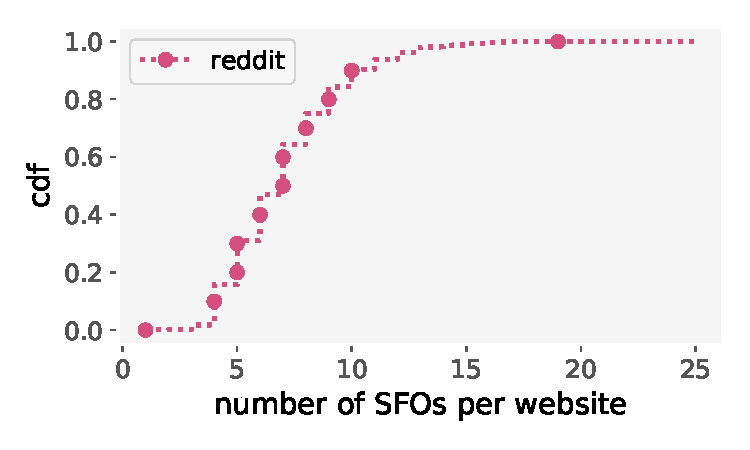
\includegraphics[width=\columnwidth]{../exp/plot/img/sfo-dist}
	\caption{%
		SFO distribution derived from the most frequently viewed reddit pages as
		of December 4, 2019.
	}
	\label{fig:sfo-dist}
\end{figure}

  \section{Discussion} \label{sec:discussion}

\subsection{Privacy}
At least mention privacy leaks to auditor. For example, related to CT logs uptime.
  \section{Design 2} \label{sec:design-log}
\begin{figure*}
    \centering
    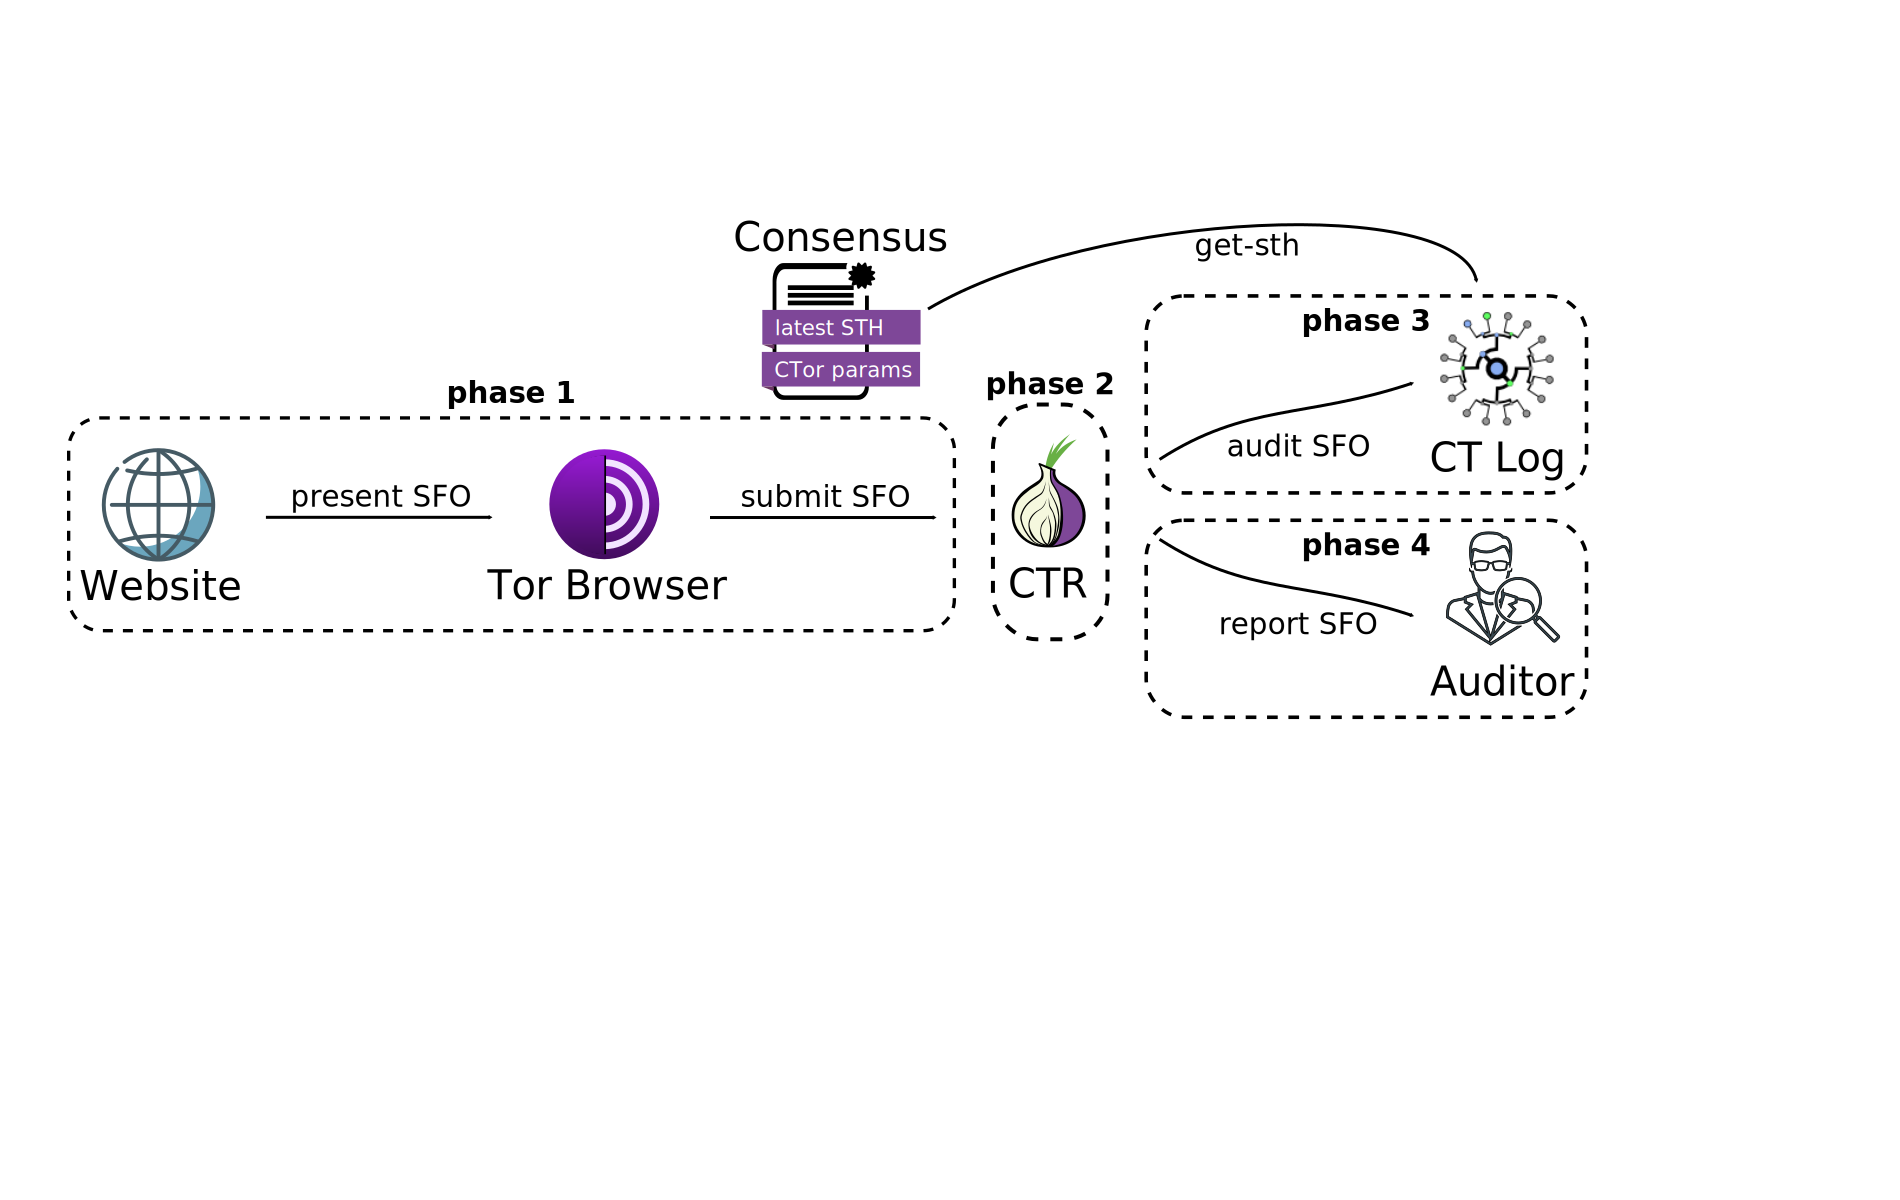
\includegraphics[width=0.85\textwidth]{img/setting-with-consensus}
    \caption{An overview of our design: Tor's consensus is extended by including
        the latest STH from each relevant CT log (periodically fetched by
        Directory Authorities) together with global CTor parameters (presented
        throughout Section~\ref{sec:design}). A website presents a SFO to Tor
        Browser, and Tor Browser in turn submits this SFO with some probability
        (consensus parameter) to a randomly selected CTR (phase 1). The CTR
        temporarily stores the SFO (phase 2). After some random delay (another
        parameter), the CTR attempts to audit the SFO by challening the issuing
        CT log using the STH in the consensus (phase 3). Upon failed audit, the
        SFO is reported to a trusted auditor listed in the consensus (phase 4).
        All connections are made over dedicated independent circuits.}
    \label{fig:overview2}
\end{figure*}
  \section{Design 2b} \label{sec:design-log}
\begin{figure*}
    \centering
    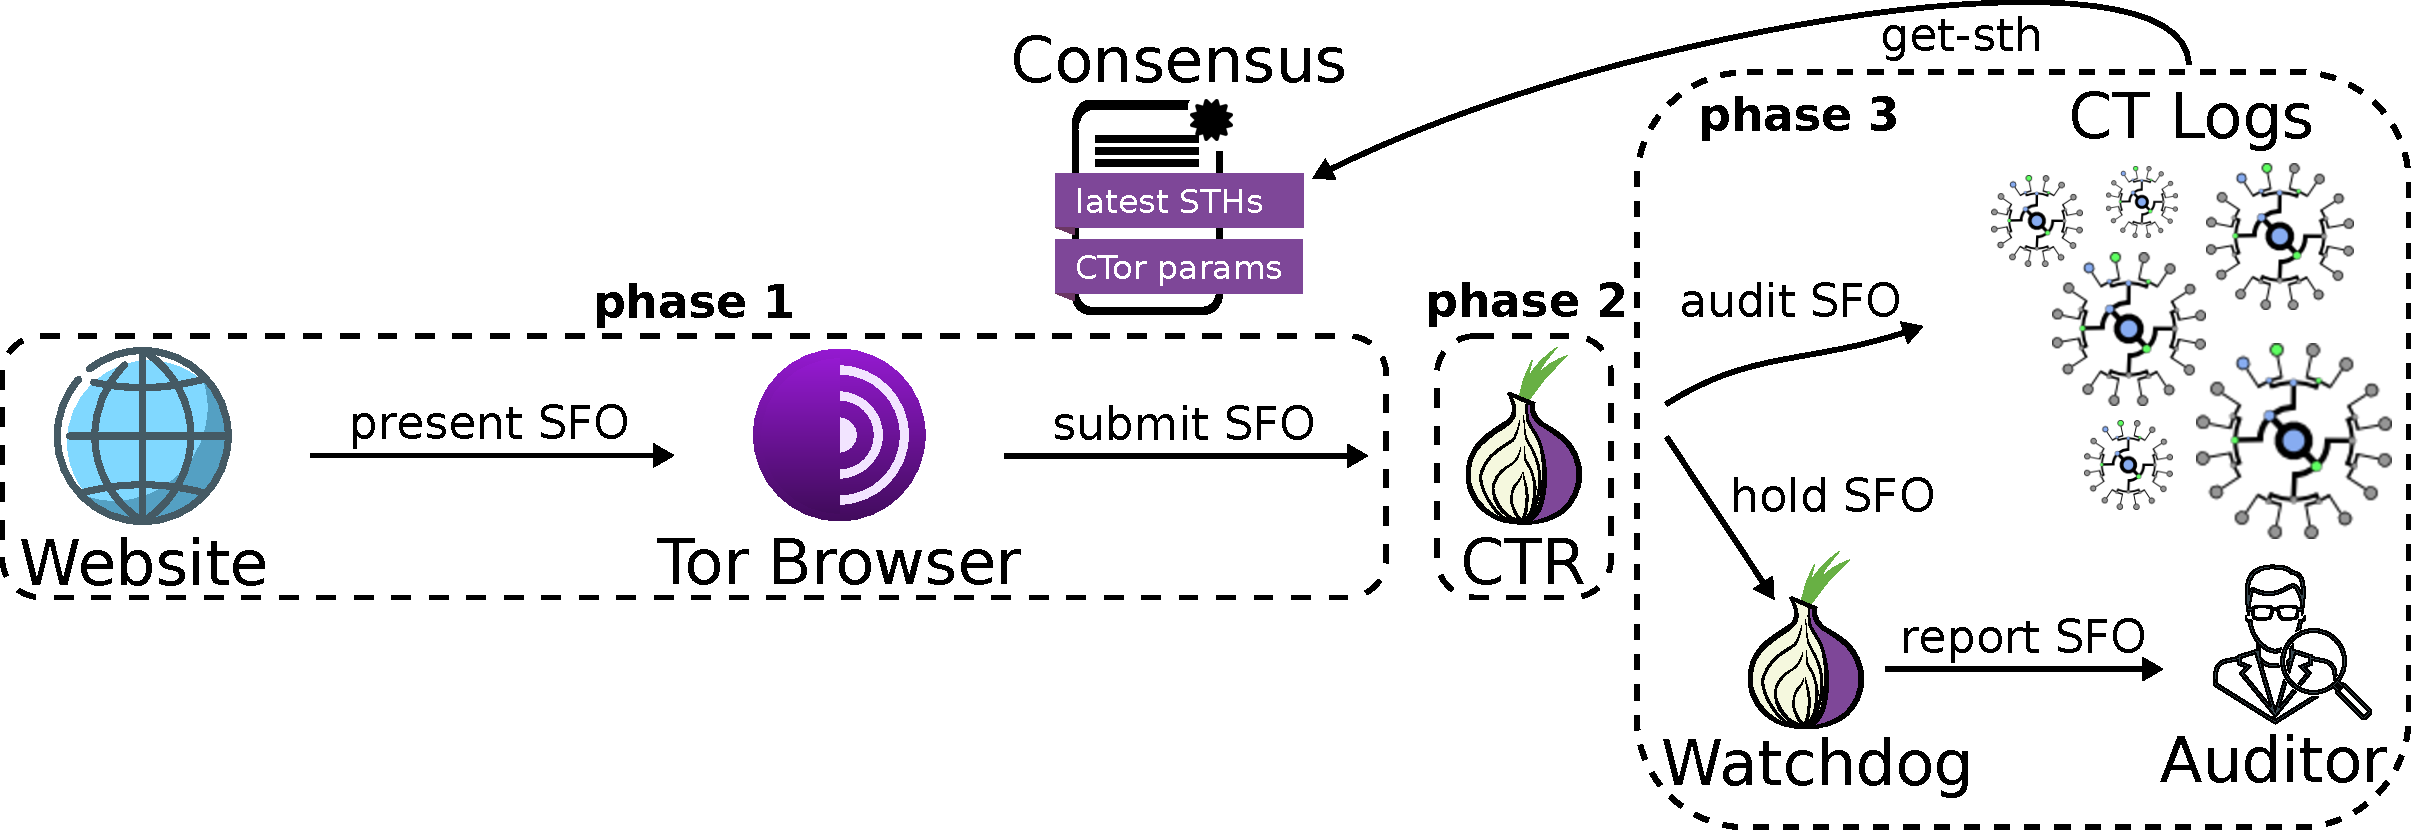
\includegraphics[width=0.85\textwidth]{img/design-auditor}
    \caption{todo}
    \label{fig:design-auditor}
\end{figure*}

  \section{Conclusion} \label{sec:conclusion}
CTor consists of a base design and two possible extensions with the goal of
adding incremental and privacy-preserving support for Certificate Transparency
to Tor. The use of relays in the Tor network distributes caching of observed
SFOs and delays interactions with CT logs, central to both overall security and
preserving privacy of Tor users. Our analysis also shows that these relays are
the weakest link: the most promising chance of avoiding exposure of compromising
SFOs appears to be to attempt to perform network-wide DoS on relays, or attack
CT logs directly. 

Mitigation of network-wide attacks take us outside of Tor's---and therefore also
our---threat model. That said, we cannot ignore such attacks given the strong
attacker we consider (to some degree in control of both a trusted CA and CT
logs). Several parameters of our design enables Tor to \emph{adapt} to observed
interference with CTor, such as a network-wide DoS of relays, reported targeted
attacks of CT logs, or relays reporting suspected flooding through the
\texttt{ct-delete-bytes}  extra-info. When it comes to TB, the submission
probability (\texttt{ct-submit-pr}) and SFO size threshold
(\texttt{ct-max-sfo-bytes}) could be set such as to force all SFOs to be sent to
a CTR before accepting any new HTTPS application-layer data. During the storage
phase, the consensus specifies each CT log's MMD and the delay distribution
(\texttt{ct-delay-dist}), which can be set to either minimize or maximize the
delay between TB user and CT log interaction. Similarly, trusted auditors
(auditor extension) and log operator relationships (base design and log
extension) are also defined in the consensus and can be tweaked.

Deploying CTor, in particular with the log extension that requires trusted
auditors, would be a significant operational burden. Overall Tor network health
would have to include considerations of tweaking CTor parameters to adapt to
strong attackers. However, the potential gains are significant. Tor users would
benefit from the significant security improvement provided by CT logs. Perhaps
more significantly, Tor would be a system for maintaining a
probabilistically-audited cryptographically-verifiable view of the entire CT log
ecosystem available from Tor’s consensus. This would benefit the wider web and
Internet, since the view from Tor's consensus could serve as a base of trust,
relaxing the necessary trust that currently has to be placed on CT log
operators. As a starting point, our base design turns Tor Browser into a helpful
participant in addressing the weakest-link issue of the CA ecosystem, in line
with the goals of CT.


  \bibliographystyle{abbrv}
  \bibliography{src/ref}

  %\appendix
  %\section{Extra}
\end{document}
